\begin{activity}{Magnetic Susceptibility of Rocks}

\section*{Purpose}

This activity links magnetic susceptibility to mineralogy and geological processes such as alteration, metamorphism, weathering, and igneous differentiation.

\section*{Learning Outcomes}

By the end of this activity, you should be able to:
\begin{itemize}
  \item Measure magnetic susceptibility on a range of rock and ore samples and record observations systematically.
  \item Relate susceptibility values to mineralogy, particularly the role of magnetite and other iron oxides.
  \item Distinguish primary (igneous) from secondary (alteration or metamorphic) controls on rock magnetic susceptibility.
  \item Discuss why susceptibility is not a simple proxy for bulk rock composition or metal content.
\end{itemize}

\section*{Background}

Magnetic susceptibility ($\chi$) describes how strongly a material becomes magnetized in response to a field:
\[
    \mathbf{M} = \chi \mathbf{H} .
\]

Unlike density, which depends on the bulk mineralogy of a rock, susceptibility is controlled almost entirely by a trace phase. Magnetite's susceptibility is orders of magnitude higher than that of the silicate minerals that make up the bulk of most rocks, so even a few percent by volume of magnetite dominates the measured susceptibility regardless of what the rest of the rock is made of. A handful of Ni- and Co-bearing minerals can also contribute, but at typical crustal abundances their effect is negligible next to magnetite's.

Because susceptibility is set by a trace phase, it is sensitive to exactly which Fe-Ti oxide is present, not simply how much iron the rock contains. Figure~\ref{fig:mag-ternary} shows the relevant Fe-Ti oxide system: magnetite and its Ti-substituted relatives at one end, hematite and ilmenite at the other. Today's samples will let you see this system in action --- the same starting rock can end up on either side of it, depending on what reaction it underwent.

\begin{figure}[h]
  \centering
  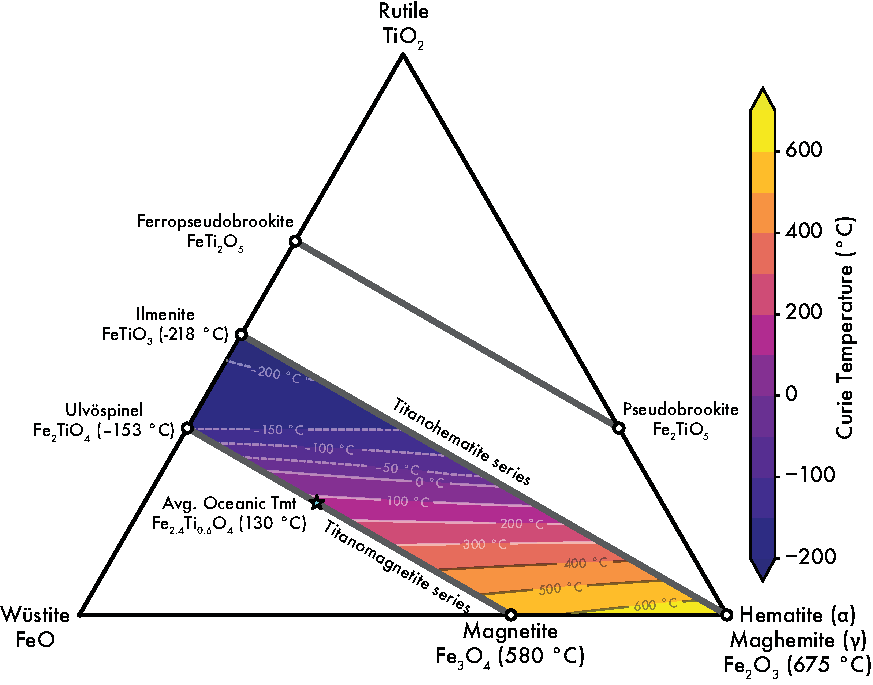
\includegraphics[]{figures/Fe_Ti_oxide_ternary.pdf}
  \caption{The Fe-Ti oxide system. Which side of this diagram a rock's oxide phase falls on --- not its bulk iron content --- determines whether it is magnetic.}
  \label{fig:mag-ternary}
\end{figure}

\section*{Samples and Observations}

\subsection*{Station 1: Reaction Pairs}

\begin{table}[h]
    \centering
    \begin{tblr}{
      colspec = {ccX[c]cX[c]},
      row{2-6} = {ht=2.5em},
      hline{1,2,7} = {solid},
      hline{3-6} = {dashed},
      vline{1,2,6} = {solid},
      vline{3-5} = {dashed}
    }
        \textbf{Sample} & \textbf{Rock type} & \textbf{Geological context} & \textbf{Susceptibility (SI)} & \textbf{Notes} \\
        1 & peridotite & & & \\
        2 & serpentinite & & & \\
        3 & basalt (fresh) & & & \\
        4 & basalt (altered) & & & \\
        5 & eclogite & & & \\
    \end{tblr}
        %6 & (granite/sedimentary protolith) & & \\
        %7 & (metamorphosed equivalent) & & \\
\end{table}

\begin{questions}
  \question{Reaction Pairs}
  \begin{enumerate}
    \item Compare the peridotite and serpentinite susceptibility. How does serpentinization lead to high magnetic susceptibility?
    \answerbox[3cm]

    \item Compare the fresh basalt and altered seafloor basalt. Why can alteration dramatically reduce susceptibility in mafic rocks?
    \answerbox[3cm]

    \item Compare the granite or sedimentary protolith with its metamorphosed equivalent. Which minerals control susceptibility in felsic or sedimentary rocks?
    \answerbox[3cm]
  \end{enumerate}

  Serpentinization of olivine is commonly associated with reactions such as
  \[
    6\,\underbrace{\ce{(Mg_{0.9}Fe_{0.1})2SiO4}}_{\text{olivine}} + 7\,\ce{H2O} \longrightarrow
    3\,\underbrace{\ce{Mg3Si2O5(OH)4}}_{\text{serpentine}} +
    \underbrace{\ce{Mg(OH)2}}_{\text{brucite}} +
    0.4\,\underbrace{\ce{Fe3O4}}_{\text{magnetite}} + 0.4\,\ce{H2}
  \]
  while oxidative weathering of basalt may involve reactions such as
  \[
    4\,\underbrace{\ce{Fe_{3-x}Ti_xO4}}_{\text{titanomagnetite}} + \ce{(1-x)O2} \longrightarrow
    6\,\underbrace{\ce{Fe_{2-2x/3}Ti_{2x/3}O3}}_{\text{titanohematite}} \, .
  \]

  \question{Cross-Comparison: Two Paths to Low Susceptibility}
  Both the altered seafloor basalt and the eclogite are weakly magnetic, but they reached that state by different geological histories. Propose one observation (mineralogical, textural, or geochemical) that could distinguish which process --- surface alteration or deep metamorphism --- produced a given low-susceptibility sample.
  \answerbox[3cm]

  \question{Cross-Comparison: One Process, Two Outcomes}
  Hydrothermal alteration acted on both the peridotite and the basalt in this activity, but with opposite magnetic consequences: serpentinization of peridotite \emph{produces} magnetite, while seawater alteration of basalt \emph{destroys} it. Given that both are altered by broadly similar fluid-rock interaction, what property of the starting rock --- rather than the process itself --- determines whether magnetite is created or consumed?
  \answerbox[3cm]
\end{questions}

\subsection*{Station 2: Igneous Suite}

\begin{table}[h]
    \centering
    \begin{tblr}{
      colspec = {ccX[c]cX[c]},
      row{2-6} = {ht=2.5em},
      hline{1,2,7} = {solid},
      hline{3-6} = {dashed},
      vline{1,2,6} = {solid},
      vline{3-5} = {dashed}
    }
        \textbf{Sample} & \textbf{Rock type} & \textbf{Predicted rank} & \textbf{Susceptibility (SI)} & \textbf{Notes} \\
        6 & gabbro & & & \\
        7 & diorite & & & \\
        8 & granodiorite & & & \\
        9 & granite 1 & & & \\
        10 & granite 2 & & & \\
    \end{tblr}
\end{table}

\begin{questions}[resume]
  \question{Igneous Suite}
  \begin{enumerate}
    \item Before measuring, rank the igneous samples from most to least magnetic based on their appearance (color index, inferred mafic mineral content).
    \answerbox[2cm]

    \item After measuring, compare your predicted ranking to the results. Does susceptibility track color index as expected? What might cause a sample to depart from the trend?
    \answerbox[3cm]
  \end{enumerate}
\end{questions}

\subsection*{Station 3: Ore Minerals}

\begin{table}[h]
    \centering
    \begin{tblr}{
      colspec = {ccX[c]cX[c]},
      row{2-4} = {ht=2.5em},
      hline{1,2,5} = {solid},
      hline{3-4} = {dashed},
      vline{1,2,6} = {solid},
      vline{3-5} = {dashed}
    }
        \textbf{Sample} & \textbf{Mineral} & \textbf{Predicted rank} & \textbf{Susceptibility (SI)} & \textbf{Notes} \\
        11 & magnetite & & & \\
        12 & galena & & & \\
        13 & tin ore & & & \\
    \end{tblr}
\end{table}

\begin{questions}[resume]
  \question{Ore Minerals}
  \begin{enumerate}
    \item Before measuring, rank the four ore samples from most to least magnetic, based on their appearance and metal content.
    \answerbox[2cm]

    \item After measuring, compare your prediction to the results. Which sample most surprised you, and why?
    \answerbox[3cm]

    \item Pyrite contains iron. Why is it only weakly magnetic, if at all, despite this?
    \answerbox[2cm]
  \end{enumerate}
\end{questions}

\section*{Complete at the end}

\begin{questions}[resume]
  \question{Synthesis}
  \begin{enumerate}
    \item Why is susceptibility not a simple proxy for bulk composition or metal content?
    \answerbox[2cm]

    \item Which geological processes and settings tend to increase susceptibility, and which tend to decrease it?
    \answerbox[2cm]
  \end{enumerate}

  \question{Reflection}
  Explain why petrology is essential for interpreting magnetic anomalies.
  \answerbox[3cm]
\end{questions}

\section*{Key Ideas}

\textbf{Magnetite controls crustal magnetization.} Because the susceptibility of magnetite is orders of magnitude higher than that of common silicate minerals, even a few percent magnetite can dominate the magnetic response of a rock. Susceptibility therefore reflects the abundance of magnetic Fe-Ti oxides rather than bulk composition or metal content. In igneous rocks, this abundance commonly decreases as melts evolve toward more felsic compositions, producing systematic variations in susceptibility across an igneous suite through primary crystallization alone. No alteration or metamorphic overprint is required to generate these magnetic contrasts.

\textbf{Sorry physics isn't the answer to everything.  Petrologic history is essential for magnetic interpretation.} Without knowing the mineralogy, alteration history, and redox evolution of the source rocks, magnetic anomalies can be highly ambiguous. The same bulk composition may produce very different magnetic responses depending on the abundance and stability of magnetic minerals such as magnetite or titanomagnetite. Likewise, processes such as alteration and metamorphism do not have a fixed effect on susceptibility: depending on the initial iron content, oxidation state, and fluid or melt chemistry, they may either create or destroy magnetic minerals. Consequently, interpreting magnetic anomalies requires an understanding of the underlying reaction geochemistry and mineralogical evolution, not simply the identification of a geological process.

\end{activity}